\documentclass[a4paper]{article}
\usepackage[margin=3cm]{geometry}
\usepackage{graphicx}

\usepackage{hyperref}
\hypersetup{
	colorlinks=true,
	linkcolor=blue,
	filecolor=magenta,
	urlcolor=cyan,
	hyperindex=true,
	linktocpage=true,%makes the page number be the link in the index
}
\usepackage{listings}
\lstset{
	basicstyle=\tiny\ttfamily,
	columns=fullflexible,
	keepspaces=true,
	breaklines=true,
	frame=single,
	showstringspaces=true,
	tabsize=4,
	showspaces=true,
	showtabs=true,
}

\renewcommand{\arraystretch}{1.2}

\title{Bit flips per operation}

\author{Chaya2766}

\begin{document}
	\sffamily
	\hyphenchar\font=-1
	\sloppy
	
	\maketitle
	
	\textbf{
		\sloppy
		\hyphenchar\font=-1
		}
	
	\vfill
	
	\begin{abstract}
		Abstract goes here
	\end{abstract}
	
	%\noindent \rule{\linewidth}{1pt}
	\vfill
	
	\tableofcontents
	
	\pagebreak
	
	\section{Assumptions}
	
	Why NAND gates?
	
	\pagebreak
	
	\section{Addition}
	\label{addition}
	
	\noindent\rule{\linewidth}{0.5pt}
	
	\noindent
	\begin{minipage}{0.4\linewidth}
		The half adder is used for the first layer of addition (ie. the first bit of both numbers) and has only 5 NAND gates.
	\end{minipage}
	\begin{minipage}{0.6\linewidth}
		\begin{center}
			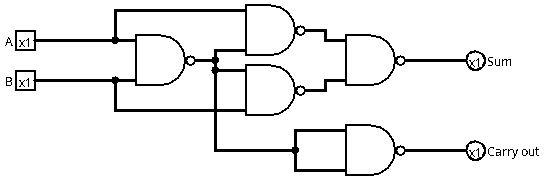
\includegraphics[width=0.6\linewidth]{circuits/half_adder.png}
		\end{center}
	\end{minipage}
	
	\noindent\rule{\linewidth}{0.5pt}
	
	\noindent
	\begin{minipage}{0.4\linewidth}
		The full adder consists of 9 NAND gates and has to be used for each next bit after the first.
	\end{minipage}
	\begin{minipage}{0.6\linewidth}
		\begin{center}
			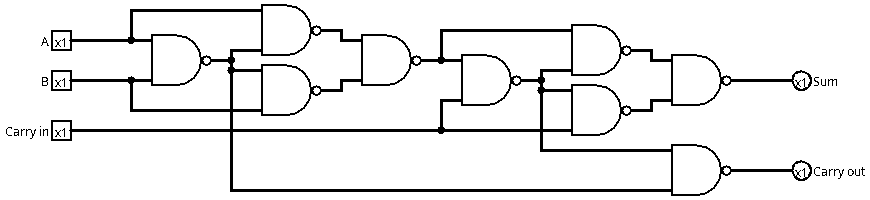
\includegraphics[width=0.9\linewidth]{circuits/full_adder.png}
		\end{center}
	\end{minipage}
	
	\noindent\rule{\linewidth}{0.5pt}
	
	Here is an example 4-bit adder with 32 NAND gates:
	
	\begin{center}
		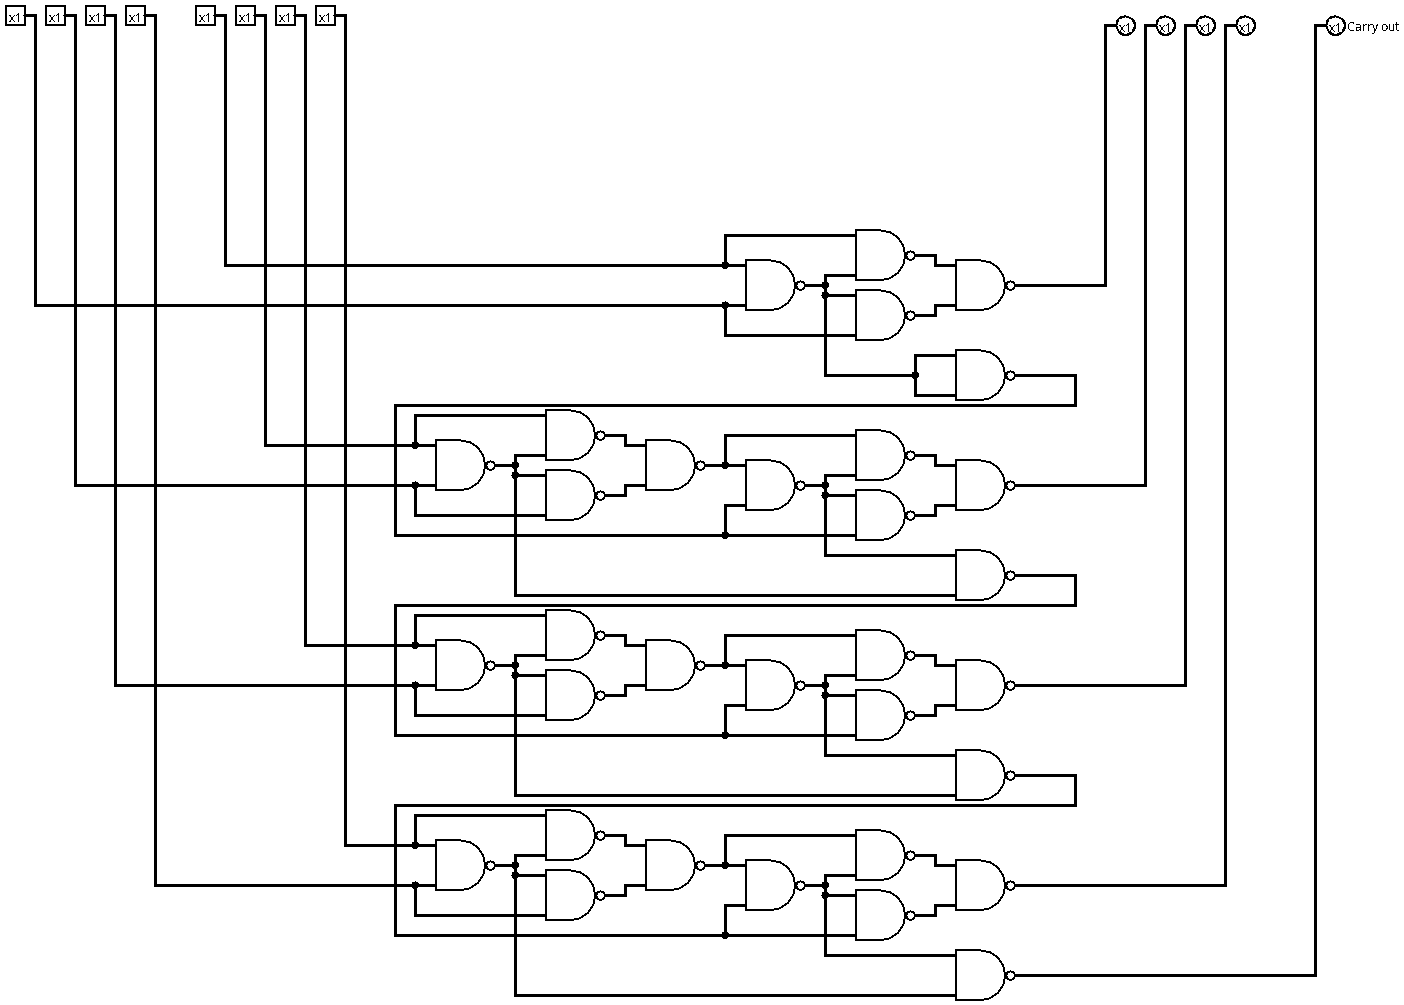
\includegraphics[width=0.9\linewidth]{circuits/4-bit_adder.png}
	\end{center}
	
	\noindent\rule{\linewidth}{0.5pt}
	
	This shows that the number of NAND gates in an adder circuit can be described as such:
	
	$$ G = 5 + (n-1)\cdot9 = 9n - 4$$
	
	where:
	
	\begin{itemize}
		\item $G$ is the number of NAND gates in the adder
		
		\item $n$ is the number of bits of the adder
	\end{itemize}
	
	One gate could also be removed in the final step if you don't need the carry bit.
    
	\pagebreak
	
	\section{Multiplication}
	
	(big thanks to this video \href{https://www.youtube.com/embed/O34KquoMpT0}{https://www.youtube.com/embed/O34KquoMpT0})
	
	\medskip
	
	The multiplier type I'll be using is simple cascading multiplier that works something like this:
	
	\begin{center}
		\begin{tabular}{c | c | c | c | c | c | c |}
			number A 	& & & & $A_2$ & $A_1$ & $A_0$ \\
			number B 	& & & & $B_2$ & $B_1$ & $B_0$ \\\hline
			partial 1	& & & & $A_2B_0$ & $A_1B_0$ & $A_0B_0$ \\
			partial 2	& & & $A_2B_1$ & $A_1B_1$ & $A_0B_1$ & \\
			partial 3	& & $A_2B_2$ & $A_1B_2$ & $A_0B_2$ & & \\\hline
			sum			& $P_5$ & $P_4$ & $P_3$ & $P_2$ & $P_1$ & $P_0$ \\
		\end{tabular}
	\end{center}
	
	$A_n$ represents the nth bit of number A, and the same for number B.
	
	$P_n$ represents the nth bit of the result.
	
	\medskip
	
	Multiplying two bits (eg. $A_0$ with $B_0$ which would be written as just $A_0B_0$) is an AND operation. Every combination of two bits requires an AND gate, which is made from 2 NAND gates. This part adds $2n^2$ NAND gates to the multiplying circuit.
	
	\medskip
	
	The additions have to be done with adders such as shown in section \ref{addition}. First row of multiplications (partial 1) does not need adders. Second row (partial 2) can start with a half-adder as well as end with a half-adder but needs full adders inbetween. The rows after that can start with a half-adder but then be full adders to the end.
	
	This means the second row adds 2 half-adders and n-2 full adders, which translates to $2\cdot5 + (n-2)\cdot9 = 9n - 8$ NAND gates.
	
	And each row from third and onwards adds $1\cdot5 + (n-1)\cdot9 = 9n-4$ NAND gates. Since in an n-bit adder there are going to be n partial rows, this gets multiplied by $n-2$.
	
	\medskip
	
	In total we need to sum up these terms:
	
	$2n^2$ from the ANDs across the whole thing.
	
	$9n - 8$ from the adders in the second row.
	
	$(n-2)\cdot(9n-4) = (9n^2-22n+8)$ from the adders from row 3 onwards.
	
	\medskip
	
	In total an n-bit adder should have this many gates:
	
	$$ G = 11n^2 - 13n $$
	
	where:
	
	\begin{itemize}
		\item $G$ is the number of NAND gates in the multiplier
		
		\item $n$ is the number of bits of the adder
	\end{itemize}
	
	\medskip
	
	\noindent\rule{\linewidth}{0.5pt}
	
	Here is an example 3-bit multiplier with 60 gates (yes I counted manually to confirm):
	
	\begin{center}
		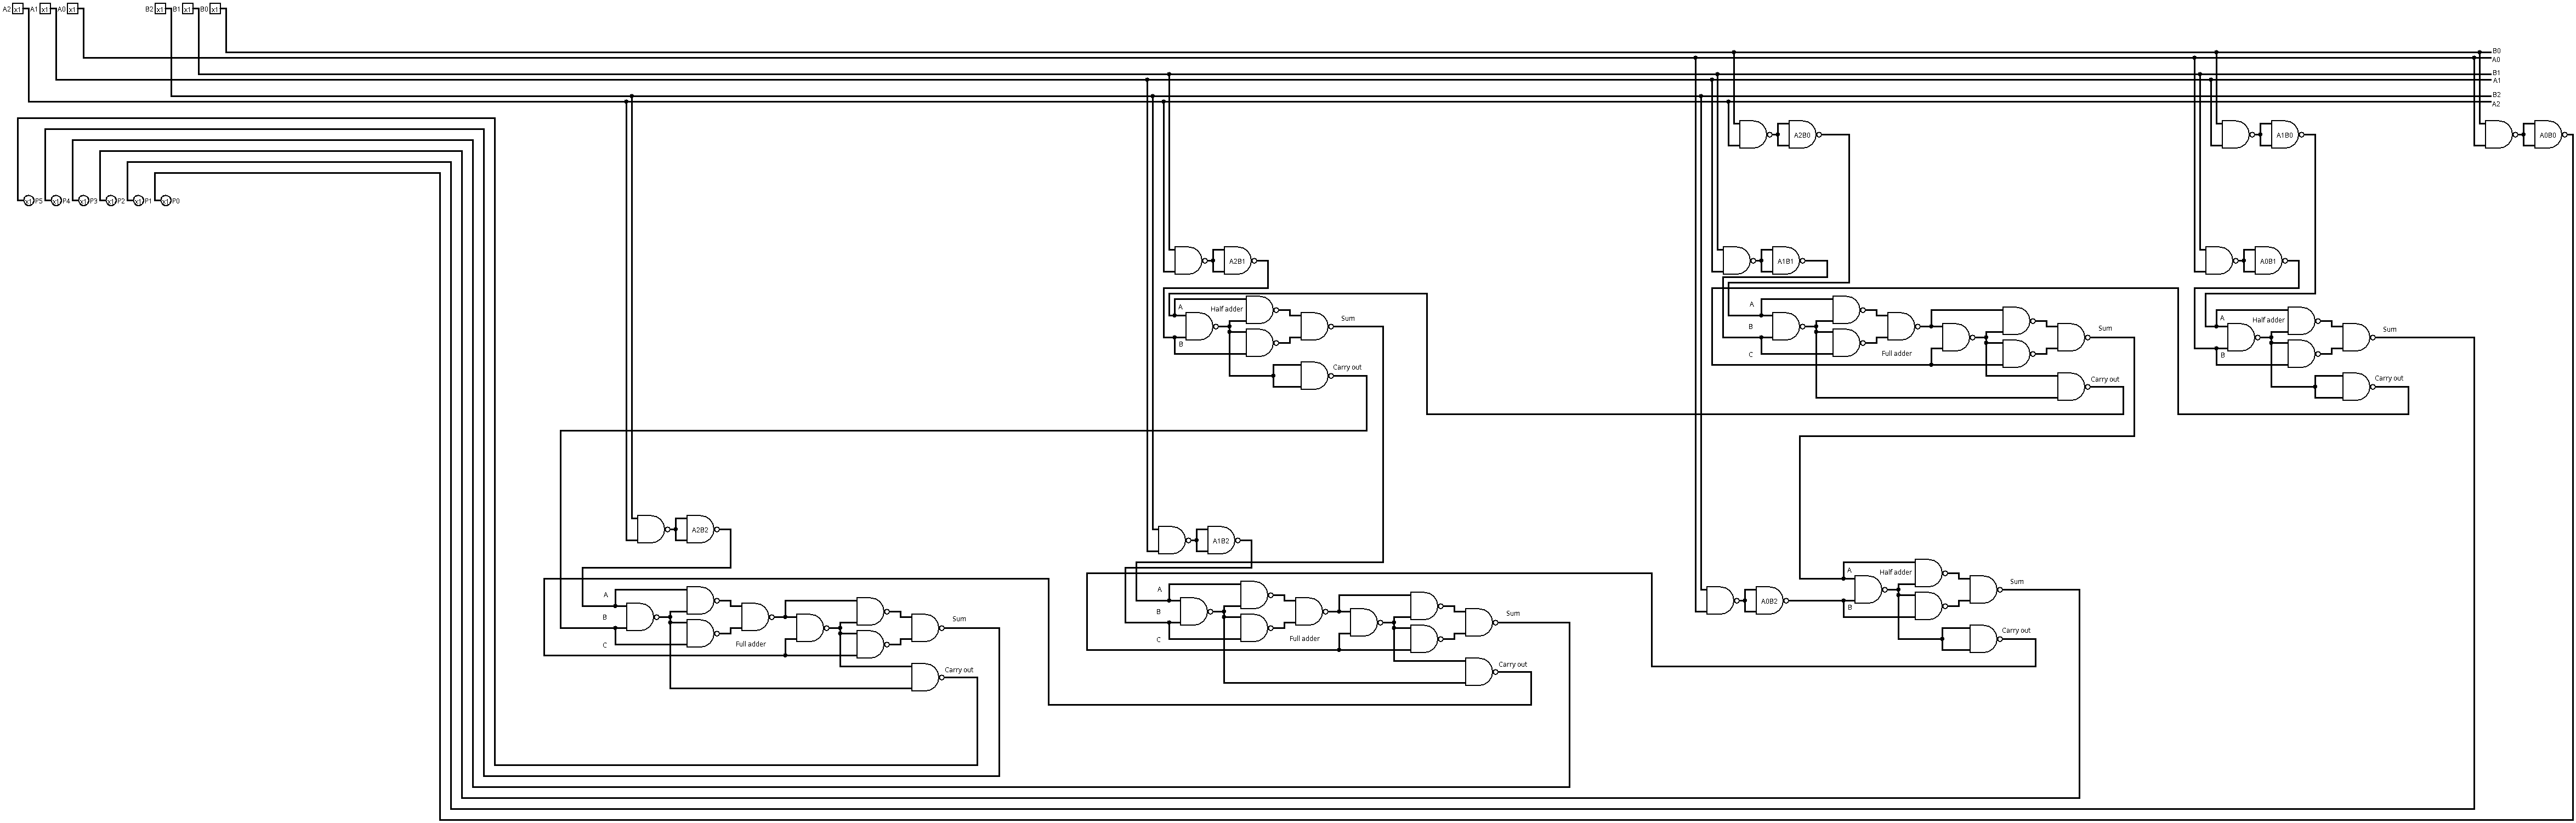
\includegraphics[width=0.9\linewidth]{circuits/3-bit_multiplier.png}
	\end{center}
	
\end{document}